% % no answer key
% \documentclass[letterpaper]{exam}

% answer key
\documentclass[letterpaper, landscape]{exam}
\usepackage{2in1, lscape} 
\printanswers{}

\usepackage{units} 
\usepackage{xfrac} 
\usepackage[fleqn]{amsmath}
\usepackage{cancel}
\usepackage{float}
\usepackage{mdwlist}
\usepackage{booktabs}
\usepackage{cancel}
\usepackage{polynom}
\usepackage{caption}
\usepackage{fullpage}
\usepackage{comment}
\usepackage{commath}
\usepackage{enumerate}
\usepackage{graphicx}

\everymath{\displaystyle}

\title{Statistics \\ Week Five}
\date{\today}
\author{}

\begin{document}

\maketitle
\tableofcontents

  \section{Equations of Lines}
  \begin{itemize*}
    \item Explain slope, y-intercept, etc.
    \item show how to get slope from two points
    \item show how to get equation from slope and one point
  \end{itemize*}

  \section{HANES Data} % (fold)

  \begin{enumerate*}
    \item find equation for SD line ($w = 14.89597 h - 832.924$)
    \item draw SD line 
    \item talk about predicting weight from height by adding corresponding SD
    \item calculate mean weights for short/tall samples. Notice that short
      people are 0.43 heaver than expected and tall people are 0.43 lighter than expected.
    \item talk about predicting weight using average weight for that height. Draw line through
      midpoint of vertical slices.
    \item draw best fit line for means
    \item calculate slope of best fit line for means
    \item notice that slope is 0.43 of SD slope. One change of SD in height results in 0.43
      change in SD for weight
    \item find equation for regression line ($w = 6.445742h - 254.929$)
  \end{enumerate*}
  
  General rule for regression line:
  \begin{itemize*}
    \item line goes through $\del{ \bar{x}, \bar{y} }$ 
    \item slope is:
      \[
        m = r \cdot \frac{s_y}{s_x}
      \]
  \end{itemize*}

  \begin{align*}
    \bar{y} & = m \bar{x} + b \\
    b       & = \bar{y} - m \bar{x} \\
  \end{align*}

  \begin{itemize*}
    \item $r$ is number of y standard deviations change for each x standard
      deviation change 

    \item $r^2$ is fraction of variation in $y$ accounted for by changes in $x$.

    \item $r = \pm 1$ for exact match

    \item $r = 0$ for no correlation.  If you change x, you don't expect any
      corresponding change in y

    \item for height/weight, $r^2 \approx 0.1872442$

    \item regression line minimizes square of differences from prediction
  \end{itemize*}

  Calculating height from weight gives a different line:
  \begin{align*}
    m & = 0.4327172 \cdot \frac{2.98}{44.39} \\
      & = 0.02904927 \\
    b & = 68.46 - 0.02904927 \cdot 185.96 \\
      & = 63.058 \\
    \\
    h & = 0.02904927 w + 63.058 \\
  \end{align*}

  Doing it this way is like drawing a line through the midpoint of the horizontal slices
  through the football.

  Questions:
  \begin{enumerate}
    \item The mean age 45--54 in the HANES sample had an average height of 69
      inches.  This is the same as the overall average height.

      T/F\@: their average weight should be around 171 lbs (overall average
      weight)?

      \begin{solution}
        False.  
        
        The average weight for people 69 inches tall is the average of a
        vertical slice over 69.  This probably will about match the overall
        average.

        However, men 45--54 don't all appear in the vertical slice over 69.
        They're scattered about the graph.  Older men tend to be heavier for
        their height, so the average weight of this group is probably higher
        than 171 lbs.

        With our data set, the correlation between age and weight for men
        between 18 and 60 is 0.2.

      \end{solution}

    \item In regression of height to weight, men who are 73 inches tall average
      176 lbs in weight. T/F\@: men who are 176 lbs average 73 inches tall?

      \begin{solution}
        False---there is a different regression equation when going the other direction.
      \end{solution}

  \end{enumerate}

  \section{Examples}
  
  \subsection{Exams} % (fold)
  
  In a class, midterm and final scores have a mean of 60 and an SD of 15.  The correlation
  between midterm and final scores is 0.5.  Estimate the average final scores for a midterm
  score of:

  \begin{enumerate}[(a)]
    \item What is the regression line for final vs.\ midterm?
      \begin{solution}
        \begin{align*}
          m  & = 0.5 \cdot 1 \\
             & = 0.5 \\
          60 & = 0.5 \cdot 60 + b \\
          b  & = 30 \\
          f  & = 0.5m + 30 \\
        \end{align*}
      \end{solution}

    \item midterm: 75
      \begin{solution}
        \begin{align*}
          f & = 0.5 \cdot 75 + 30 \\
            & = 67.5 \\
        \end{align*}
      \end{solution}

    \item midterm: 30
      \begin{solution}
        \begin{align*}
          f & = 0.5 \cdot 30 + 30 \\
            & = 45 \\
        \end{align*}
      \end{solution}
      
    \item midterm: 60
      \begin{solution}
        \begin{align*}
          f & = 0.5 \cdot 60 + 30 \\
            & = 60 \\
        \end{align*}
      \end{solution}
  \end{enumerate}

  Notice that people who did well on the midterm do less well on the final and people who did
  poorly on the midterm to better on the final. This is regression to the mean.

  \subsection{SAT} % (fold)
  
  For some school:
  \begin{tabular}[H]{lrr}
         & mean & SD \\
    SAT  & 550  & 80 \\
    GPA  & 2.6  & 0.6 \\
  \end{tabular}

  $r = 0.4$

  \begin{enumerate}[(a)]
    \item Find the equation for the regression line which predicts GPA based on SAT.\@

      \begin{solution}
        \begin{align*}
          m   & = 0.4 \cdot \frac{0.6}{80} \\
              & = 0.003 \\
          2.6 & = 0.003 \cdot 550 + b \\
          b   & = 0.95 \\
          gpa & = 0.003 sat + 0.95 \\
        \end{align*}
      \end{solution}

    \item
      What is the expected GPA for a student with an SAT score of 650?

      \begin{solution}
        \begin{align*}
          gpa & = 0.003 \cdot 650 + 0.95 \\
              & = 2.9 \\
        \end{align*}
      \end{solution}

    \item
      What is the expected GPA percentile for a student in the 95th
      percentile for SAT scores?

      \begin{solution}
        convert to z-score: $z_{SAT} \approx 1.644854$

        Convert to SAT score:
        \begin{align*}
          z   & = \frac{x - \bar{x}}{s} \\
          x   & = z \cdot s + \bar x \\
          \\
          sat & = 1.644854 \cdot 80 + 550 \\
              & \approx 682 \\
        \end{align*}

        calculate expected GPA:\@ 
        \begin{align*}
          gpa & = 0.003 \cdot 682 + 0.95 \\
              & \approx 3.0 \\
        \end{align*}

        convert back to percentile:
        \begin{align*}
          z & = \frac{3.0 - 2.6}{0.6} \\
            & \approx 0.6667 \\
        \end{align*}

        This is around the 75th percentile.

      \end{solution}
  \end{enumerate}

  \section{Residuals}

  \begin{itemize}
    \item A residual is the difference between the predicted and actual value.

    \item Scatter plot of residuals (x value vs.\ residual) looks like random
      cloud of points. Any change in $y$ caused by a change in $x$ is gone.

    \item sum of residuals always zero

    \item Regression line minimizes R.M.S. error of residuals:
      \[
        \text{error} = \sqrt{\frac{\sum r_i}{n}}
      \]

    \item Approximate RMS for residuals is $\sqrt{1 - r^2}$.

    \item RMS for residuals is similar to $s$ for sample (draw picture with
      error shading around regression line). 
      \begin{itemize*}
        \item About 65\% of residuals are less than one error
        \item About 95\% of residuals are less than two errors
      \end{itemize*}

    \item If you use the line $y = \bar{y}$ as the regression line (ignore any
      effect $x$ has on $y$ and guess that a $y$ value is likely to be the
      average value of $y$), then the RMS of the residuals is equal to the
      standard deviation.

    \item Error:
      Improvement over using $y = \bar{y}$ as the regression line is measured by
      multiplying $s$ by $\sqrt{1 - r^2}$.

      \[
        e \approx s_y \sqrt{1 - r^2}
      \]

      \begin{itemize*}
        \item $r = \pm 1$: error goes to zero.
        \item $r = 0$: no improvement---error is same as $s_y$
        \item $r$ somewhere in between gives an improvement
      \end{itemize*}

    \item $r^2$ is measure how much regression explains variation in y based on
      variation in x.

  \end{itemize}

  \begin{table}[H]
    \centering
    \begin{tabular}{rrrrrrrr}
      \toprule
      x & 1 & 2 & 3 & 4 & 5 & 6 & 7 \\ 
      y & 1 & 2 & 3 & 5 & 4 & 6 & 7 \\ 
     \bottomrule
    \end{tabular}
  \end{table}

  \begin{align*}
    s_y                & = 2.1602 \\
    r                  & = 0.9643 \\
    rms                & = 0.5722 \\
    s_y \sqrt{1 - r^2} & = 0.5722 \\
  \end{align*}


  \section{Outliers}

  \subsection{Middle}

  Outliers in middle of x range don't have much effect because the line can't
  move to accommodate them.  $r$ doesn't change much because high $z_y$ is
  multiplied by $z_x$ close to zero.

  \begin{figure}[H]
    \centering
    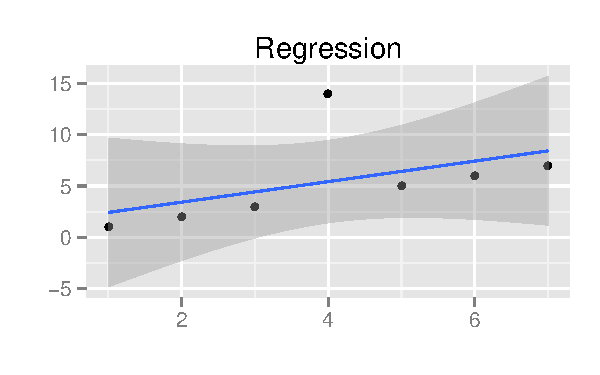
\includegraphics{figures/middle_outlier.pdf}
    \caption{Outlier in Middle}
  \end{figure}

  $r = 0.4962168$

  \subsection{End}

  Outliers at end of x range have large effect because the line can move to
  accommodate them.  
  
  $r$ decreases dramatically because high $z_y$ is multiplied by
  large negative $z_x$.

  \begin{figure}[H]
    \centering
    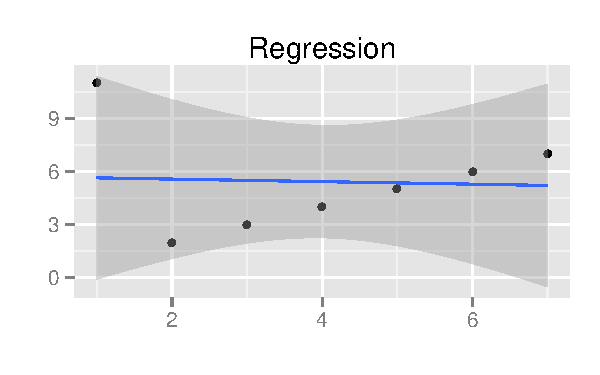
\includegraphics{figures/end_outlier.pdf}
    \caption{Outlier at End}
  \end{figure}

  $r = -0.05157106$

  \subsection{Middle Outlier}
  \begin{itemize*}
    \item outliers in middle of x range don't have much effect because the line can't
      move to accommodate them

    \item outliers at either end of the x range have a big effect because the line
      moves to fit them in
  \end{itemize*}

  \section{Regression to the Mean}
  For any repeated test, people tend to be closer to the mean on the second
  attempt.

  \subsubsection{Heights of Fathers vs.\ Heights of Sons} % (fold)

  \begin{itemize}
    \item draw graph with oval, father height on the x-axis
    \item draw graph with standard deviations instead of heights
    \item draw vertical slice at tall fathers. Sons of tall fathers tend to be
      shorter than their father (regression to the mean)
    \item draw vertical slice at short fathers. Sons of short fathers tend to be
      taller than their father (regression to the mean)
  \end{itemize}
  
  \subsection{Other Examples} % (fold)
  
  \begin{itemize*}
    \item pilots with bad/good landings and instructor criticism/praise.
    \item retake of standardized tests
  \end{itemize*}

\end{document}

